\documentclass[12pt]{article}
\usepackage[utf8]{inputenc}
\usepackage{float}
\restylefloat{table}
\usepackage{amsmath}
\usepackage{tikz}
\def\checkmark{\tikz\fill[scale=0.4](0,.35) -- (.25,0) -- (1,.7) -- (.25,.15) -- cycle;}


\usepackage[hmargin=3cm,vmargin=6.0cm]{geometry}
%\topmargin=0cm
\topmargin=-2cm
\addtolength{\textheight}{6.5cm}
\addtolength{\textwidth}{2.0cm}
%\setlength{\leftmargin}{-5cm}
\setlength{\oddsidemargin}{0.0cm}
\setlength{\evensidemargin}{0.0cm}
\setlength{\parskip}{1em}

%misc libraries goes here
%\usepackage{fitch}


\begin{document}

\section*{CENG435 - Term Project Report (Part 2) } 

\section*{Student Information }

Name : Orçun Başşimşek \\
Id Number : 2098804 \\
\\

\section{Introduction}

\ \ \ \ In this project, I developed "Reliable Data Transfer" (RDT) protocol over a UDP with Java programming language. This part of the term project consists of 2 parts. For first part, I implemented reliable transmission with pipelining. For second part, I also included multi-homing implementation. Details are explained in next sections.

\section{Implementation Details of First Experiment}

\ \ \ \ For the first experiment, I transmitted given large file (5MBytes) over the shortest path that I found at part 1 of term project. The shortest path was \textbf{S - R3 - D}. Thus, I implemented my scripts for just these three nodes for this part. I also used two helper class named \textbf{Packet} class and \textbf{CheckSum} class. These two classes are used at each node.

\subsection{Packet Class}
\ \ \ \ I used this class to box my UDP packets. As expected, I designed my packets as 1000 bytes in total (header + payload). I used first 20 bytes for header fields, and remaining 980 bytes for payload (data) for each packet object. The general view of my packets as follows.



\begin{table}[H]
  \centering
    \begin{tabular}{|l l|}
    \hline
    Type (header)   & 4 bytes     \\
    Length (header)   & 4 bytes     \\
    Sequence Number (header)   & 4 bytes     \\
    Checksum (header)   & 8 bytes     \\
    Data (payload)   & 980 bytes     \\
    \hline
    \end{tabular}%
    \caption{General View of my Packets}
\end{table}%

Type field is just an integer that can hold 0,1 or 2. Type 0 packets are my normal 1000 bytes packets that carry payload from "input.txt". Type 1 packets are just header sized (20 bytes) packets and their responsibility is just replying successful messages with ACK numbers (for this type of packets Sequence Number field is used for ACK No). Type 1 packets are only sent by destination node which is D normally. Finally, type 2 packets are only used for termination processes of my scripts. Termination mechanism of my node scripts will be explained later in detail. Length field just represents the length of total packet length in bytes. Sequence number field represents sequence number for type 0 packets( payload packets that sent from source node S), and this field also used for ACK Number for type 1 packets that sent from destination node D. Finally, Checksum field carries inverted checksum that is calculated by source node S with the help of \textbf{Checksum} class. Checksum calculation and methods of this class are going to be explained in next subsection.

Besides these attributes, Packet class has just helper getter and setter methods to dealing with raw data extracted from DatagramPackets'. At the sender side, I used getBytes() method of this class to make our packets ready to send over DatagramSocket with DatagramPackets, and at the receiver side, I used static getPacket() method of this class to reach header fields and payload data from received DatagramPackets' basically.

\subsection{CheckSum Class}
\ \ \ \ I created this class for implementing checksum calculation and checking purposes at the receiver node D. I took checksum as 8 bytes long field in my packet structure as described above. Actually, this field only represents the 16 bits binary number as a checksum for me. To fit this number in a variable, and make the header allocation for checksum in packet structure more rigid, I prefer send it in a long type variable. My real checksums are just length of 16 strings like "1001011001110001". The main method of this class is "calculateChecksum(byte[] array)" method. In this method, to calculate checksum from my payload coming from "input.txt", I firstly created sum variable as 0 which is equal to "0000000000000000". Then, from byte[] array coming from file, I converted each value of this array to a binary number as well and added it to my sum variable. This binary addition is done from "binaryAddition()" method of this class, and at the end if there is a carry bit, I also add it to the result to get correct result of the checksum. 

For the usage of this class, at the sender side, node S uses "makeInvertedChecksum()" method of this class. This method just invert the bits of calculated checksum described above. Then, node S convert this length of 16 String to a long variable and put it the going packet's header's checksum field. At the receiver side, node D firstly extracts this long variable from checksum field of received packet, and then convert it to a 16 length of String named as \textbf{Received Checksum}. And then, from received packet, it also calculates checksum from payload byte[] array by using "calculateChecksum()" method again, and it gives the name \textbf{Calculated Checksum} to it. Then, node D simply add them by using "binaryAddition()" method.
\begin{center}
$Sum \ Of \ Checksums = Calculated \ Checksum + Received \ Checksum$
\end{center}

As a result, after finding \textbf{Sum of Checksums}, it controls each bit of it. I know that if the packet is received without any corruption, this result must be equal to "1111111111111111". Hence, if there is any "0" bit in the Sum of Checksums, there is an error in the received data. In this case, node D simply discard the received packet(do not write it to "output.txt"), and send ACK for lastly successfully received packet instead of this packet. At the end, one of the main rules of reliability which is \textbf{"ensuring the correction of the received data"} is achieved with this class.   



\subsection{MainSenderNodeS and SenderSource Classes}

\ \ \ \ These classes run at the source node S. MainSenderNodeS class is just the runner class which contains main() methods of this node. It just creates the instance of SenderSource class which does real job. For the first part, I know that I have only one route which is \textbf{S - R3 - D}. Thus, this node just communicates with R3 node directly.

For SenderSource class, its "start()" method is called from runner main() method and, sending the file from this node is started. Basically, SenderSource class runs two seperate threads that have also some important shared resources. First of these threads is responsible for sending payload packets, and whose general algorithm is implemented in the "start()" method. Second of these threads is responsible for receiving ACK packets from node D (over R3 of course). I used \textbf{ArrayDeque} class of Java as my sender side buffer for \textbf{buffering}. I also needed to a sliding window concept to implement one of the pipelining approach. For this purpose, I simply used \textbf{Semaphore} class of Java which is actually used for lock mechanisms, but for my case, besides its help of making our application thread-safe, I used the Semaphore to control the size of sliding window. One more advantage of using Semaphore is that I can decide the ACKed and NON-ACKed packets at the sliding window by using "acquire()" and "release()" methods of it. Besides these fields, of course I need to thread-safe "base", "nextSequenceNumber" fields to handle my ACK/NACK mechanism in my queue (sender buffer). These are "volatile" fields, and any change of it is directly seen from both of two threads I mentioned above. Moreover, to provide reliability, I also needed to \textbf{retransmission} of lost or corrupted packets. In this project, I chose the \textbf{go-Back-N} protocol among the pipelined protocols. Thus, I also kept one \textbf{Timer}, and implemented "run()" method of TimerTask class with \textbf{1 second} timeout for oldest unACKed packet. In every 1 second, all packets in the window is retransmitted if it is not restarted from any point of application.

For working details of mentioned two threads, the first thread which is responsible for sending payload packets from "input.txt" file does its job mainly inside the "start()" method of SenderSource class. It simply creates the timer, creates the second thread which is responsible for receiving ACK packets, and creates an instance of Checksum class for creating checksum header field of going packets. Then, it goes inside the infinite while loop, and main action is done in this loop. It starts to read 980 bytes from "input.txt" file at each iteration. Then, it simply creates checksum for this specific 980 bytes payload and prepare the packet for sending process. Because this packet is unACKed yet, it acquires a permit from Semaphore (i.e. sliding window in our case). And also, include this packet into the queue (sending buffer). Then, it sends the packet to R3 node. Finally, it controls if there is a unACKed packet in window, it restarts the timer and increments the nextSequenceNumber field by one. After that, it waits the termination of second thread which is receiveACK thread, and it also terminates itself. Termination process for all scripts are same. Thus, it is going to be explained in detail later.

For working of second thread which is responsible for receiving ACK packets, after initial configurations, it starts to wait coming ACK packets. When it receives the packet, it fetches the Sequence Number Field which is used for ACK number at this type (type 1) of packets as I mentioned in Packet class section. Then, it calculates the number of received packets. Here, I thought that it is unnecessary to hold any expected ACK number field because some ACK responses may be lost, but after some loses, if I got an ACK for a packet greater than the base number of window, I understood that previous payload packets were also received successfully by destination node D. For example, if I got ACK for packet 25, and then I got ACK for packet 29, I simply understood that pakcet 26-27 and 28 also received successfully from node D. Thus, when I got ACK for packet 29 after packet 25, I can simply mark packet 26-27-28-29 as ACKed in my buffer. From this thought, this thread calculates the number of received packets, and deletes them from the queue, also releases their places from sliding window. After that, it updates the base number according to lastly ACKed packet number. Finally, if there is no unACKed packet in the queue, it cancels the timer. If there is unACKed packet in the queue, it just restarts the timer for first thread. As a one more note, besides Semaphore class, I used timerLock and queueLock objects to prevent using corresponding shared resources at completely same time by threads.


\subsection{NodeR3 and Router Classes}
\ \ \ \ These classes run at the R3 node. This node simply works as router. It is greatly taken from my first part codes with a little bit additions. Multi-threading concept is also used for this node. NodeR3 class just has runner main() method, and it creates two threads. One of them is for receiving payload packets from node S, and sending them to node D. And, another one is for receiving ACK packets from node D, and sending them to node S. Send and receive processes implemented in "run()" method of Router class simply as I did in part 1 of term project.

\subsection{MainReceiverNodeD and ReceiverDestination Classes}
\ \ \ \ These classes run at the destination node D. Node D is basically responsible for receiving the payload packets, writing them to "output.txt" file in order and sending corresponding ACK packet for each successfully received payload packet. MainReceiverNodeD class has just runner main() method for node D. It creates an instance of ReceiverDestination class by supplying output file name, and communication informations for node R3 (because node D directly communicates with node R3 only). And then, it just calls the start() method of this object. \\

For ReceiverDestination class, it is main class for this node that does the real job. Importantly, it has Checksum object for checksum checking, and FileOutputStream object to write payload to "output.txt" file. It also has \textbf{expectedSequenceNumber} field. It is used for correct ordering of received packets. Its aim is similar to "nextSequenceNumber" field of source node S as explained above. In the start() method of this class, node D starts to wait payload packets. After receiving a packet, it firstly fetches the Type header of packet, and checks it. If it is type 2 packet (i.e. termination packet), it simply terminates itself. If it is type 0 packet (i.e. payload packet), it controls the data corruption by using the Checksum header field of received packet and using methods of Checksum class as explained in Checksum Class section. It also controls the Sequence Number header field of packet. If it is equal to "expectedSequenceNumber" and data is also not corrupted, it simply process the given packet, and write its payload to our "output.txt" file. And then, it sends ACK to source, then increases the expectedSequenceNumber field by one. If received packet is not expected packet in order or data corruption occurs on packet's payload, node D simply sends ACK for lastly successfully received packet again.

Lastly, port informations for S-R3-D nodes at first part is as follows: \\
For S-R3-D payload flow: S (port = 1060) - R3 (port = 1080) - D (port = 1090) \\
For D-R3-S response ACK flow: D (port = 1090) - R3 (port = 1070) - S (port = 1060) \\



\section{Implementation Details of Second Experiment}

\ \ \ \ For the second experiment, I transmitted given large file over the remaining two paths between node S and node D at the same time. The remaining paths for me are \textbf{S - R1 - D} and \textbf{S - R2 - D} paths. I used same code templates for node S and node D with some additions for \textbf{multi-homing} and \textbf{detecting link failure}. For R1 and R2 nodes, I used totally same node R3 script from experiment 1 scripts.


\subsection{Implementation of Multi-homing} 
\ \ \ \ I implemented this multi-homing approach basically by using multi-threading in my source node S and destination node D scripts from experiment 1. Here, I have two paths which are S - R1 - D and S - R2 - D. 

Firstly, for source node S script, I decided to use two seperate threads for each of these paths. However, in experiment 1, I also used two threads for source node as I mentioned. One of them is for sending payload data, and other one is receiving ACK responses. These two threads already works on a one path. Therefore, in total, I decided to use 4 threads to handle sending and receiving operations of 2 paths simultaneously. As in experiment 1, two threads are working on S - R1 - D path, and another two threads are working on S - R2 - D path. They have same key attributes and operations as in experiment 1 basically. One of the main change is that, for these two paths I used same buffer and sliding window, and I increased the window size capacity from 10 to 20. All of 4 threads reach the shared resources through some lock mechanisms to prevent any race conditions. For this time, I also have a lock for FileInputStream instance, to guarantee that sending payload threads read data from "input.txt" in turn, not exactly at same time. The only unshared fields are socket information and receiver informations for each of these 2 paths.

For destination node D, I have used only 1 thread that communicates with R3 node in experiment 1. However, this time, I also used multi-threading in node D. One thread communicates with S thread over R1 router, and other thread communicates with S thread over R2 router. These two threads again have shared FileOutputStream with lock mechanisms, they have thread-safe and shared expectedSequenceNumber field also, to guarantee that two threads know the any differences about expected packet number information immediately.   


\subsection{Implementation of Link Failure Detection}
\ \ \ \ For detecting link failure, I know that my DatagramSocket.receive() method is blocking method, and if there is a no coming packet, it is going to block forever by default. From this point, I thought that I could set some timeout (for example 10 seconds) for my sockets (i.e. I change the blocking time of DatagramSocket.receive() method from default infinity to 10 seconds by using "setSoTimeout()" method of DatagramSocket) when waiting packets. If there is no packet coming within 10 seconds when the code is blocking in DatagramSocket.receive() method, it simply throws "SocketTimeoutException". And then, I catch this exception and terminate the all threads (sender S, router, receiver D) through the downed link.



\section{Termination Mechanism of Scripts}
\ \ \ \ For termination, I used two different mechanisms to ensure termination. Firstly, I thought using type 2 packets. Type 2 packets is just header sized packets, their only non-trivial header field is \textbf{Type} field. In general, when a node observes that it receives a packet with type 2, it knows that it means End-Of-File for transmission. After that, it also informs neighbour node about the ending of file transmission. All nodes get this type of packet at the end, and they terminates themselves properly.

Secondly, when thinking link failure detection for experiment 2, I also thought that "setSoTimeout()" could also be used for termination of live links. Again I used same 10 seconds wait for this purpose here. I did that because sometimes type 2 packets may be down. Thus, after waiting 10 seconds, if there is no incoming message, all nodes again terminates themselves. \\
\\

Lastly, port informations for two paths at second part is as follows: \\
\\
For S-R1-D payload flow: S (port = 1115) - R1 (port = 1140) - D (port = 1120) \\
For D-R1-S response ACK flow: D (port = 1120) - R1 (port = 1130) - S (port = 1115) \\
\\
For S-R2-D payload flow: S (port = 1145) - R2 (port = 1170) - D (port = 1150) \\
For D-R2-S response ACK flow: D (port = 1150) - R2 (port = 1160) - S (port = 1145) \\


\section{Experiment Results for Part 1}
\ \ \ \ First of all, I run my experiment 1 scripts without adding any delay or loss to links. I checked that receiver node D receives the file \textbf{as it is}, and I saw the complete (5 Mb) and correct file at the receiver side at the end of file transmission without any problem. File transmission lasted \textbf{20 seconds} without adding any delay or loss to links. Some screenshots from execution are below.

\begin{figure}[h!]
  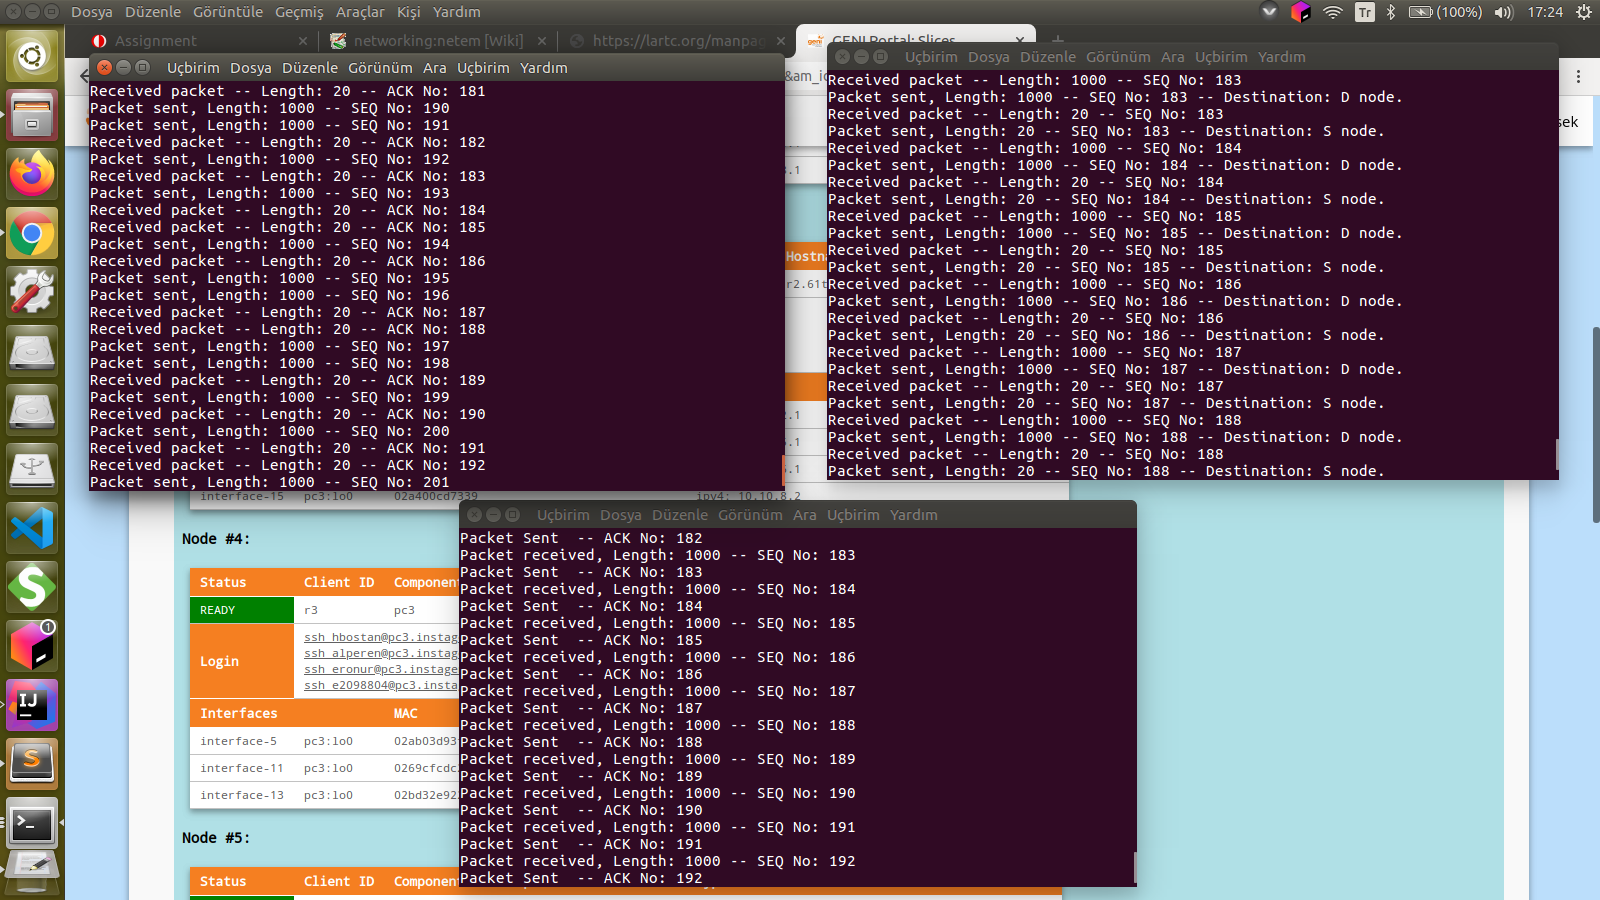
\includegraphics[width=\linewidth]{e1start.png}
  \caption{Working of nodes for first part}
\end{figure}

In figure 1, left-above terminal belongs to node S, right-above terminal belongs to node R3 and below terminal belongs to node D. At the below figure (Figure 2), termination of all of three nodes can be seen.

\begin{figure}[h!]
  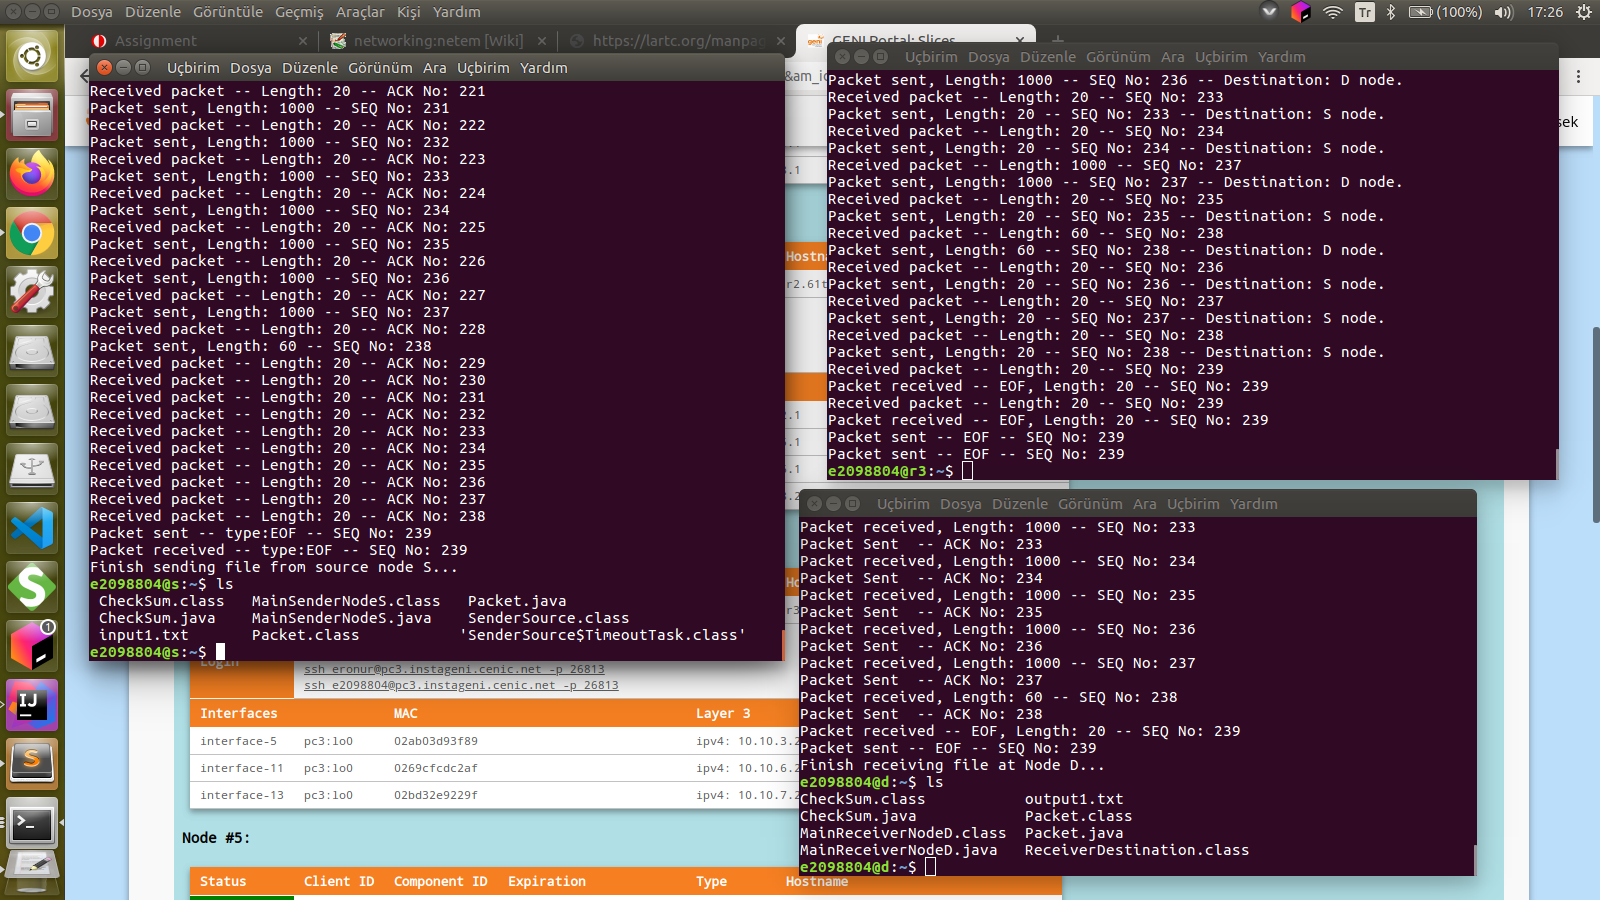
\includegraphics[width=\linewidth]{e1fin.png}
  \caption{Termination of nodes for first part}
\end{figure}

After that, I conducted first step of the experiment and I added \textbf{3 ms} delay and \textbf{5\% loss} to all links of S, R3 and D. Even though it lasts only 20 seconds without adding any delay and loss, for this time file transmission duration was very huge. And, it lasted \textbf{5596 seconds} and terminated properly for this step.

Secondly, I conducted second step of the experiment and I added \textbf{3 ms} delay and \textbf{15\% loss} to all links of S, R3 and D. For this time, file transmission duration was \textbf{7640 seconds} and terminated properly again for second step. Thirdly, I conducted third step of the experiment and I added \textbf{3 ms} delay and \textbf{38\% loss} to all links of S, R3 and D. For this time, file transmission duration was \textbf{15841 seconds} and terminated properly again for third step.

My results were very huge when adding delays and losses to links. Therefore, I could not conduct the experiment steps several times. Graphical representation of the results can be seen below.

\newpage

\begin{figure}[h!]
  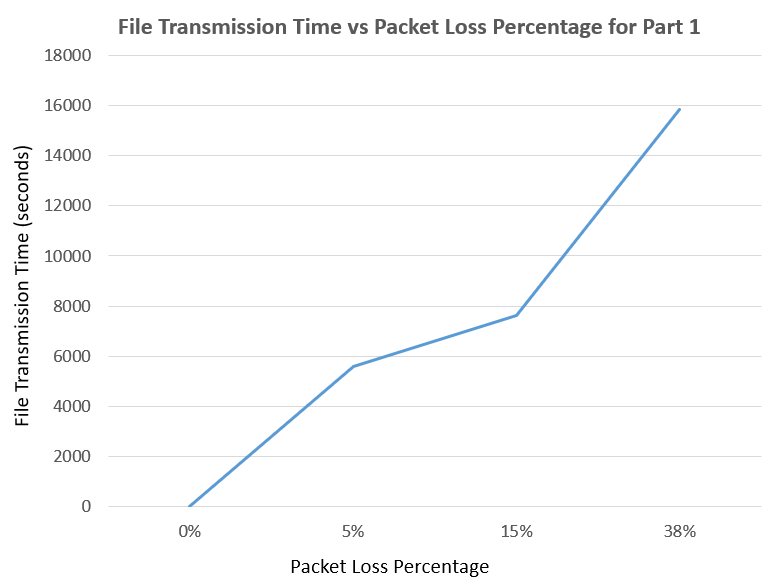
\includegraphics[width=\linewidth]{graphExp.png}
\end{figure} 


I observed that while adding more packet loss percentage to links, file transmission time is affected hugely and it increases hugely as expected. I also observed that when I add these packet losses in every step, my receiver node D script works much more slower than my sender node S script. I clearly saw that node S always waits some time for receiving ACK from node D over R3. As I mentioned, I took 10 sized buffer on sender side, and I saw that node S always tries to send a packet whose sequence number is equal to \textbf{lastly ACKed packet's sequence number + 10}. This 10 is coming from my window size at the sender side of course. However, I did not use any buffering and sliding window approach on receiver side D. Node D just sends ACK when it sees a succesful received message. In other words, due to lack of buffering in receiver node D, node D handles the packets one by one, and I thought that this is the reason for huge differences between no packet loss case and packet loss cases. If I also implemented a buffering mechanism for node D, probably I can get more consistent results. However, at the end, also by considering a no packet loss case (20 seconds case), for all 4 steps of the experiment, file transmission time increase is consistent with my applied configurations.


  


\end{document}

​

